 % Useful: http://docs.latexlab.org

\documentclass[11pt]{article}
% used by \maketitle :
\title{DarkChat: a light weight, [almost] serverless, push-based, peer-to-peer chat protocol}
\author{Nathan Griffith and Ahmet Aktay}
\date{May 12, 2010}
% used by \begin{code}:
\usepackage{fancyvrb}

\usepackage[utf8]{inputenc}
\usepackage[usenames,dvipsnames]{xcolor}
\usepackage{fullpage}
\usepackage[upright]{fourier}
\usepackage{tkz-graph}
\usetikzlibrary{arrows}


\DefineVerbatimEnvironment{code}{Verbatim}{fontsize=\small}
\DefineVerbatimEnvironment{example}{Verbatim}{fontsize=\small}
\newcommand{\ignore}[1]{}

\begin{document}
\maketitle % automatic title!

\section{Abstract}

The purpose of this project is to create a protocol for clients on a network to function with very little dependence on a server. In the case of \emph{DarkChat}, the clients function as `chat' clients. The clients are able to communicate with each other information such as `online'/`offline' state and lists of contacts, with little-to-no interaction with the server.

While \emph{DarkChat} relies on a multi-threaded approach, and also makes no use of authentication, implementation decisions such as this have been made independently of the underlying protocol. As such, the protocol could be implemented in any number of ways, and this is meant as merely one example.\footnote{For instance, the event-based, stateless nature of the protocol would make an asynchronous IO implementation a good choice in terms of resource utilization.}

\section{Clients and Servers}

The `Client' class has been built as a wrapper for the messaging and interface classes, putting them all together into one usable chat client. Note that the term `client' is slightly misleading, as with the inclusion of a simple flag, a client can function as a server with very few implementation changes. It is possible that this could be reduced even further, such that servers could simply act as `super-clients' which store information about the entire network, instead of about only their nearby edges and nodes.
In either case, the only purpose of the server is to act as a secondary or backup repository for storing information about the network. Once the network is fully operational, the server is not needed, as long as enough clients remain online that one cluster of edges does not become separated from any other. In other words, the server is a client that has been flagged as having access to greater bandwidth and resources, and can shoulder a bigger burden in maintaining network topology. It has no additional logic and hence is not a liability.

\subsection{Usage: Parameters}

A number of parameters can be passed to the client upon execution. With the exception of `username' (`-u'), all parameters will revert to default values if no value is specified. (see {\bf Figure \ref{params}}.)

\begin{figure}
\caption{Parameters that can be passed to `client.'}
\begin{code}
-p [port number, for accepting incoming communication]
-t [the default number of listening threads]
-u [the username of the client]
-sip [ip address of known server]
-sp [port number of known server]
-s (server flag, specifying that this instance of DarkChat is a server)
\end{code}
\label{params}
\end{figure}

Before a network is formed, a server may be necessary to provide a `seed' for the network topology. As such, the server IP and port number are important when first building a network that is to use this protocol.

\subsection{Usage: Macros}

Once the client has been started, a number of macros have been made available to give the user control of the the chat environment. (See {\bf Figure \ref{macros}}.)

\begin{figure}
\caption{The list of available macros, listed when `\textbackslash help' is entered}
\begin{code}
  \help
   -Display this dialog
  \chat <username>
   -Switch to conversation with <username>
  \users
   -See a list of KNOWN users (online or off)
  \online
   -See a list of known, ONLINE users
  \offline
   -See a list of known, OFFLINE users
  \add <username>
   -Attempt to add username to list of known users
  \ping <ip> <port>
   -Attempt to ping the ip at the given port
   -If no port is specified, the current instance's incoming will be used
  \explode
   -ask every adjacent node to notify every adjacent node that this user is 
    online at this address.
  \quit or \exit
   -Leave the program gracefully
\end{code}
\label{macros}
\end{figure}

The listed macros are made available before the client has necessarily made successful contact with a server or other clients, allowing one to use the `\textbackslash ping' macro to manually connect to another client or server.

Once a connection has been made, information about offline and online users should propagate across the network and to the client, at which point the macros `\textbackslash online', `\textbackslash offline', and `\textbackslash users' will provide useful information.

To communicate with an online user, one need only use the `\textbackslash chat' macro (followed by the user's name) to start a new chat session with that user. From that point on, any line of text that is entered and does not start with a macro `\textbackslash' will be sent to \emph{all online sessions} associated with the receiver's username.\footnote{Currently there is no way to chat with \emph{only one} session if a user is logged into multiple.}

The `\textbackslash explode' macro acts as a proof-of-concept for the propagation of information across nodes. While quite expensive for the network, this macro attempts to broadcast and propagate its IP address to all adjacent nodes \emph{via all short paths}. This will ensure that every node in that zone will have a significant probability of receiving this information. With little optimization, the node could broadcast this declaration to a set of users within a short bounded distance without much unneeded redundancy. 

In the case of `\textbackslash explode', if each node has n outgoing links, notifying a sphere of nodes with distance $\leq$ 2, would notify n$^2$ users in O(n$^2$) time. The node would then get n$^2$ responses back, acquiring information about n$^2$ users. In general, network traversal remain cheap as long as they stay within short-range clusters, which occur naturally in social communications, and also can reflect the physical hardware topology of the network\footnote{Users in a cluster are more likely to be `stranded' in the same island in the event of network failure.}. Hence streamlined versions of actions like `\textbackslash explode' can keep the topology regenerating without relying on the (potentially offline) central server.

\section{The Algorithm}

While the details of the `Chat' client are useful in understanding some aspects of this algorithm, the true implementation has been abstracted from the end-user. 

\subsection{The Network}

Rather than envisioning a network as comprised of `users,' `buddies' and `servers,' one can conceive of a network as an undirected graph composed of nodes and edges. Each node represents a `client.' Each edge represents a direct, two-way association between two clients.\footnote{In the context of `chat,' adjacent nodes might represent ``buddies.''}

\begin{figure}
  \caption{An example network configuration}
  \begin{center}
  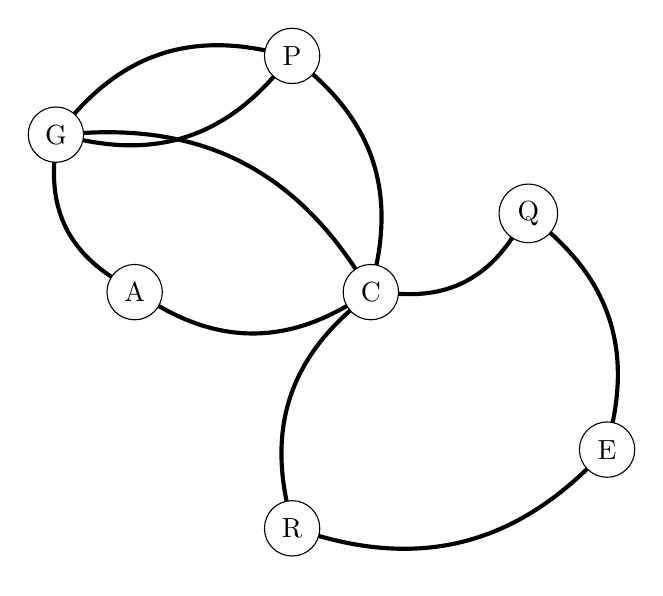
\begin{tikzpicture}
    \tikzstyle{VertexStyle}=[shape = circle, fill = white, minimum size = 20pt, text = black, draw]
    \SetUpEdge[lw         = 1.5pt,
                       color      = black,
                     labelcolor = white,
                      labeltext  = red,
                      labelstyle = {sloped,draw,text=blue}]
   \tikzstyle{EdgeStyle}=[bend left]
   \Vertex[x=0, y=4]{G}
   \Vertex[x=1, y=2]{A} 
   \Vertex[x=3, y=5]{P}
   \Vertex[x=4, y=2]{C}
   \Vertex[x=6, y=3]{Q}
   \Vertex[x=7, y=0]{E}
   \Vertex[x=3, y=-1]{R}
   \Edges(A,G,P,C)
   \Edges(Q,E,R,C,A)
   \Edges(P,G,C)  
   \Edges(Q,C)
  \end{tikzpicture}
  \end{center}
\label{graph}
\end{figure}

As shown in {\bf Figure \ref{graph}}, a network graph might look like one or more node clusters\footnote{This could be particularly true in the case of a `chat' client.}. In the \emph{DarkChat} implementation, each node must keep track of all nodes that are within two edge traversals.

When a node changes state, it sends a notification to all nodes in its list of relevant nodes. For example, if nodes \emph{R} and \emph{E} have lost their connection to each other\footnote{This might happen if they have both changed IP addresses since their last communication}, \emph{Node C} or \emph{Node Q} could facilitate the re-establishment of the connection\footnote{Of two nodes, only one need know the other's location for a connection to be established. In sending a message to \emph{Node R}, \emph{Node E} necessarily reveals its location.}.

In such a network graph, one might think that a node like \emph{Node C} would make a good location for a server. However, in a serverless setting this node simply has \emph{server-like} capabilities, by nature of its close connection to many other nodes. In this way, a server-free graph can maintain robust and redundant connections between nodes.

Because \emph{DarkChat} is not entirely serverless, all nodes would presumably be connected to some centralized server. However, only in cases where nodes are completely stranded would nodes \emph{need} to poll the server in order to maintain an accurate representation of their surrounding nodes. The more interconnected the clusters of nodes, the `healthier' the network stays as individual nodes come and go.

\subsection{The Status}

While each node's online/offline status is stored at each linked node, even offline nodes are remembered in session variables and kept. Since most end-users use the same network connections consistently through time (static IP at home and work), this information can be used to `jump-start' the connectivity of the network without invoking the central server. A balance has to be struck between iterating through (potentially useless) old addresses for nodes when attempting to reach them, and pruning the oldest away to streamline the process. In this implementation, we prune the list of sessions on demand to a desired length, favoring online sessions (however many) over those that are offline.
   
\subsection{The Protocol}

Clients make use of a limited number of message types to send and receive information. In the \emph{DarkChat} implementation, a separate set of threads constantly monitors for incoming connections, such that activity can occur in the background, regardless of the state of the user interface. (See {\bf Figure \ref{protocol}} for the list of message types.)

\begin{figure}
\caption{The underlying message types available in this protocol.}
\begin{description}
\item \emph{declareOnline} - sends a message to a specified user notifying it of the sender's online state.
\item \emph{declareOffline} - declares to the specified user that the sender is going offline.
\item \emph{requestPing} - requests that, if the receiving node can connect to a different, specified node, the receiving node forward the sender's connection information to the specified node.
\item \emph{requestUserList} - asks the receiver to reply with a list nodes adjacent to the sender (or some other specified node)
\item \emph{deliverKnownList} - deliver a list of node adjacencies to another node
\end{description}
\label{protocol}
\end{figure}

\section{Use Cases}

\emph{DarkChat} is not intended for networks that require high bandwidth and experience frequent changes in topology. It saves bandwidth for the \emph{server} by distributing the traffic workload to the clients, even to the point of being largely server-independent. While perhaps not appropriate for all uses, this protocol is particularly useful when redundancy and independence from centralized servers are more important than network efficiency.

\emph{DarkChat} has the useful property of running serverless \emph{even when the server is available}, which might be considered by many systems to be a `failure' mode (requiring backup and recovery because the server has gone down). This creates an interesting advantage for the protocol: All failsafes, backups and system load are tested (and ideally refined) during regular uptime activity, instead of being put to the test only on system failure.

\section{Comparisons}

When compared to heavy-hitting infrastructures like Microsoft's Partition and Recovery Service\cite{prs}, we see that \emph{DarkChat}-like protocols leave a lot to be desired in terms of precise and 100\% accurate recovery of data. On the other hand, systems like PRS have the advantage of designing the hardware and network layout from the ground up, while \emph{DarkChat} is built to run on available (non-enterprise) network architectures. In the event of failure, while PRS will focus on recovering data integrity, DarkChat will aim to maximize connectivity across its network topology. To this end it sacrifices the requirement that \emph{everything} be restored, or that all nodes stay fully synchronous, choosing instead to maintain more general network stability.

\section{Conclusion}

Although the \emph{DarkChat} protocol might not be right for all use cases, it in many ways has the flexibility to withstand catastrophic failures, because 100\% recovery is not a requirement. Consider a hypothetical use: coordination amongst first responders in case of an emergency. The nodes wishing to communicate will be physically close, and getting \emph{any} message through in any manner possible will be the only priority. The network DarkChat is running on might fragment into disconnected pieces entirely, but each piece will still maintain its internal topography as intact as possible and continue to ping the `missing' users in case connectivity has been restored. A fragmented set of nodes is still significantly better than none.
   
\begin{thebibliography}{1}

  \bibitem{prs}
    Atul Adya, John Dunagany, Alec Wolman,
    \emph{PRS: A Reusable Abstraction for Scaling Out Middle Tiers in the Datacenter}.
    Microsoft Research; Microsoft Corporation,
    2008.
\end{thebibliography}
\end{document}             % End of document.

